%!TEX program = xelatex
\let\stop\empty

\documentclass[12pt,a4paper]{exam-zh}

\usepackage{xeCJK}
\setCJKmainfont{Noto Serif CJK SC}
\usepackage{geometry}
\usepackage{array}
\usepackage{tikz}
\usepackage{chemfig}
\usepackage{amsmath}
\usepackage{wrapfig}
\usepackage{adjustbox}
\usepackage{enumitem}
\usepackage{fancyhdr}
\usepackage{pgfplots}
\pgfplotsset{compat=1.18}
\usetikzlibrary{calc,angles,quotes}

\usepackage{scalerel}
\def\mcirc{\mathbin{\scalerel*{\circ}{j}}}
\def\msquare{\mathord{\scalerel*{\Box}{gX}}}
\geometry{margin=2cm}

\AtBeginDocument{\zihao{4}}
% ----------- 调整 exam -----------


%region exam setup
\examsetup{
    % problem/label = \arabic*., 
    % 设置大题题号格式 
        question = {
        top-sep = 1em,      % 题头上方的间距（默认 0.25em）
        bottom-sep = 1em,   % 题号下方的间距（默认 0pt）
    },
    % 隐藏大题后的分值显示 
    problem/show-points = false,
    % 调整小题列表的缩进和间距
    list/step-name = {}, 
    solution = {
    show-solution = show-move, % 答案自动移动到卷末
    label-content = {answer},  % 答案区的标题文字
    show-qed = true            % 在解答末尾显示结束符号 ◻ 
  },
    page = {
    size = a4paper,           % 设定纸张大小 
    foot-content = { - ; - }  % 页脚显示为 -1-, -2- 格式 
  }
}
\setlist[enumerate,1]{
    label=(\alpha*), 
    itemsep=0.5em, 
    leftmargin=2em, 
    after=\hfill % 配合您之前要求的百分比靠右样式
}
\newlist{questionparts}{enumerate}{1}
\setlist[questionparts]{
    label=(\alph*),
    itemsep=0.5em,
    leftmargin=2em,
    rightmargin=4em
}
\newcommand{\qscore}[1]{%
    \unskip\nobreak\hfill
    \makebox[0pt][l]{\makebox[4em][r]{(#1\%)}}%
}
\newcommand{\solutionlayout}{%
    \setlength{\abovedisplayskip}{0.6em}%
    \setlength{\belowdisplayskip}{0.6em}%
    \setlength{\abovedisplayshortskip}{0.35em}%
    \setlength{\belowdisplayshortskip}{0.35em}%
    \setlength{\jot}{0.35em}%
}
%endregion




\begin{document}


%example1 
\chemfig{
 H_3C-[:72]{\color{blue}N}*5(- 
*6(-(={\color{red}O})-
{\color{blue}N}(-CH_3)-
(={\color{red}O})-
{\color{blue}N}(-CH_3)-=)--
{\color{blue}N}=-)}


%example2
\[
\text{化简}\quad
\left(\sqrt[3]{x^2y}\right)^2
\times
\left(\sqrt[6]{\frac{y^2}{x}}\right)^2
\]

%example3
%region 范围：弧度制——扇形弧长与面积 | 考点：扇形周长与面积的关系 | 难度：中等
\begin{question}
    如图 1 所示，扇形 $OPQ$ 以 $O$ 为圆心，且 $\angle POQ = 0.8$ rad。已知该扇形的周长为 $42$ cm，求扇形 $OPQ$ 的面积。

    \begin{center}
        \begin{tikzpicture}[scale=1.4]
            \coordinate (O) at (0,0);
            \coordinate (P) at (3,0);
            \coordinate (Q) at ({3*cos(45.84)},{3*sin(45.84)});

            \draw (O) -- (P);
            \draw (O) -- (Q);
            \draw (P) arc[start angle=0, end angle=45.84, radius=3];

            \fill (O) circle (1.5pt) node[below left]{$O$};
            \fill (P) circle (1.5pt) node[below right]{$P$};
            \fill (Q) circle (1.5pt) node[above right]{$Q$};

            \pic[draw,"$0.8\text{ rad}$",angle radius=8mm,angle eccentricity=2.4]{angle=P--O--Q};
        \end{tikzpicture}
    \end{center}

    \begin{choices}
        \item $80.7 \text{ cm}^2$
        \item $90 \text{ cm}^2$
        \item $99.3 \text{ cm}^2$
        \item $100.7 \text{ cm}^2$
    \end{choices}
\end{question}

\begin{solution}
    扇形 $OPQ$ 中，$\angle POQ = 0.8$ rad，周长为 $42$ cm，求其面积。 \\
    扇形周长由两条半径与一段弧长组成，即 $P = 2r + r\theta$；面积公式为 $A = \dfrac{1}{2}r^2\theta$。 \\
    设扇形半径为 $r$ cm。
    \begin{align*}
        2r + r(0.8) &= 42 \\
        2.8r &= 42 \\
        r &= 15
    \end{align*}
    \[
        A = \frac{1}{2}(15)^2(0.8) = 90
    \]
    故选 B。
\end{solution}
%endregion

%region 范围：直线方程与图像 | 考点：由直线方程求x、y截距判断图像 | 难度：基础
\begin{question}
    下列哪一个图像正确表示方程 $-2x+3y+6=0$？\paren[B]

    \begin{choices}
        \item
            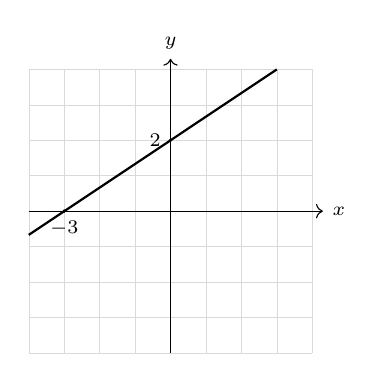
\begin{tikzpicture}[scale=0.45]
                \draw[very thin,gray!30] (-4,-4) grid (4,4);
                \draw[->] (-4,0)--(4.3,0) node[right]{\scriptsize $x$};
                \draw[->] (0,-4)--(0,4.3) node[above]{\scriptsize $y$};
                \draw[thick] (-4,-0.67) -- (3,4);
                \fill (-3,0) circle (1.5pt);
                \fill (0,2) circle (1.5pt);
                \node[below] at (-3,0) {\scriptsize $-3$};
                \node[left] at (0,2) {\scriptsize $2$};
            \end{tikzpicture}

        \item
            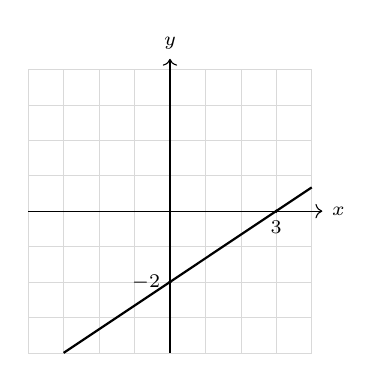
\begin{tikzpicture}[scale=0.45]
                \draw[very thin,gray!30] (-4,-4) grid (4,4);
                \draw[->] (-4,0)--(4.3,0) node[right]{\scriptsize $x$};
                \draw[->] (0,-4)--(0,4.3) node[above]{\scriptsize $y$};
                \draw[thick] (-3,-4) -- (4,0.67);
                \fill (3,0) circle (1.5pt);
                \fill (0,-2) circle (1.5pt);
                \node[below] at (3,0) {\scriptsize $3$};
                \node[left] at (0,-2) {\scriptsize $-2$};
            \end{tikzpicture}

        \item
            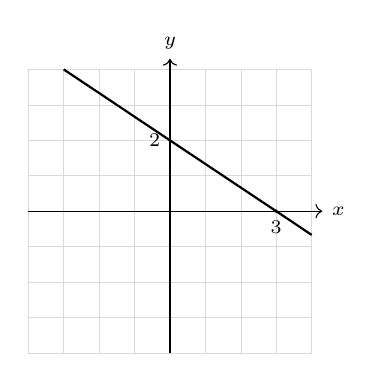
\begin{tikzpicture}[scale=0.45]
                \draw[very thin,gray!30] (-4,-4) grid (4,4);
                \draw[->] (-4,0)--(4.3,0) node[right]{\scriptsize $x$};
                \draw[->] (0,-4)--(0,4.3) node[above]{\scriptsize $y$};
                \draw[thick] (-3,4) -- (4,-0.67);
                \fill (3,0) circle (1.5pt);
                \fill (0,2) circle (1.5pt);
                \node[below] at (3,0) {\scriptsize $3$};
                \node[left] at (0,2) {\scriptsize $2$};
            \end{tikzpicture}

        \item
            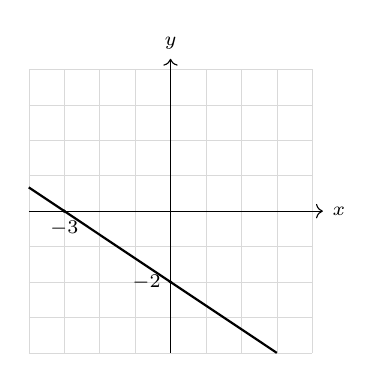
\begin{tikzpicture}[scale=0.45]
                \draw[very thin,gray!30] (-4,-4) grid (4,4);
                \draw[->] (-4,0)--(4.3,0) node[right]{\scriptsize $x$};
                \draw[->] (0,-4)--(0,4.3) node[above]{\scriptsize $y$};
                \draw[thick] (-4,0.67) -- (3,-4);
                \fill (-3,0) circle (1.5pt);
                \fill (0,-2) circle (1.5pt);
                \node[below] at (-3,0) {\scriptsize $-3$};
                \node[left] at (0,-2) {\scriptsize $-2$};
            \end{tikzpicture}
    \end{choices}
\end{question}

\begin{solution}
    求方程 $-2x+3y+6=0$ 所对应的图像。 \\
    分别令 $y=0$ 与 $x=0$ 求出两截距，再依据两截距确定图像上的点。
    \begin{align*}
        y=0: \quad -2x+6 &= 0 \\
        x &= 3
    \end{align*}
    \[
        x=0: \quad 3y+6 = 0 \ \Rightarrow \ y = -2
    \]
    该直线经过 $(3,0)$ 与 $(0,-2)$ 两点，故选 B。
\end{solution}
%endregion


\end{document}